\section{System Design}

\subsection{Model Choice}

Based on the requirements analysis and literature review, the system will be
designed around a YOLO11 object detection model, fine-tuned for the task of
luggage and people detection in surveillance footage. This model has
demonstrated strong performance on small object detection in the work by
\citet{abandoned2025vrsalovic}, making it a suitable choice for the target
application. Ease of optimisation for edge deployment on NVIDIA hardware is
also a critical factor in this choice with YOLO models being widely supported
by TensorRT optimisations (See~\ref{sec:tensorrt_optimisations}).

However, another state-of-the-art implementation of the YOLO architecture,
YOLO26, will also be evaluated as part of the model selection process. As
YOLO26 is a much more recent model, potential for improved accuracy and
efficiency is expected, but the lack of evaluations in literature may make it a
less certain choice for the final system. Evaluating both models will provide
valuable insight into their performance when compared on the test datasets, and
their suitability for edge deployment. Ultralytics themselves claim that YOLO26
is a leap forward compared to older models as seen in their own benchmarks
(figure~\ref{fig:ultralytics_benchmarks}), but these claims will be
independently verified in the context of this project.

\begin{figure*}[!htb]
	\centering
	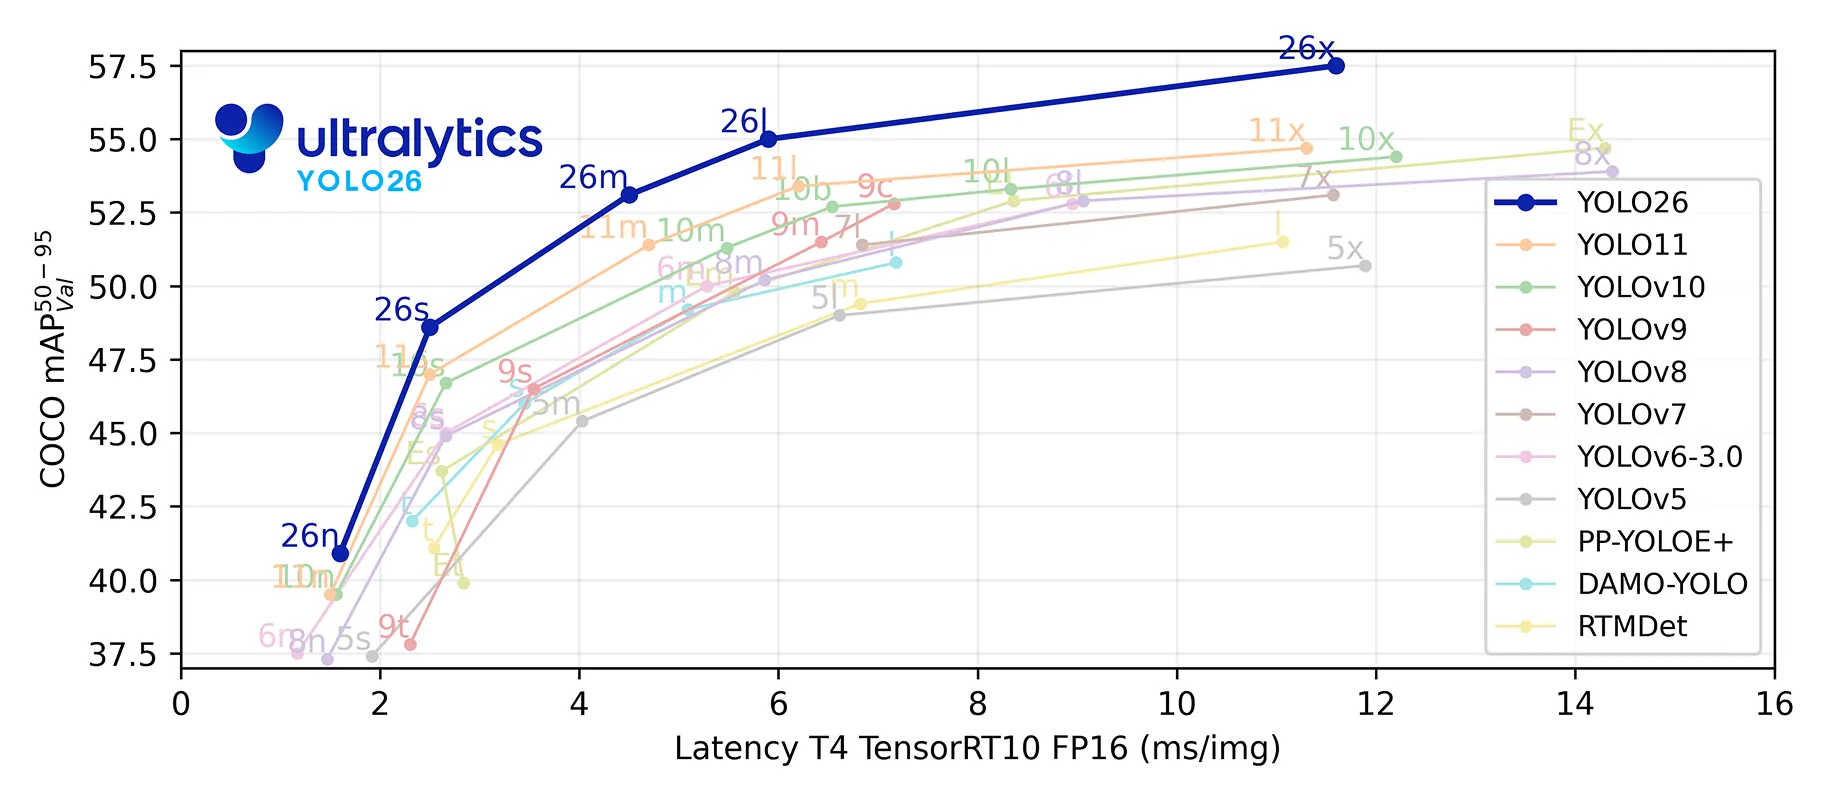
\includegraphics[width=0.8\textwidth]{figures/ultralytics_benchmarks.png}
	\caption{Ultralytics' benchmarks comparing pre-trained YOLO26, YOLO11, and older models from an article by \citet{vina2026yolo26}.}
	\label{fig:ultralytics_benchmarks}
\end{figure*}

The size of the model will be determined based on the constraints of the
hardware and the result of comparative evaluations. The nano, small and medium
variants of both models will be evaluated with the final choice being based on
the best balance of accuracy and inference speed on the target hardware.

\subsection{Tracking Algorithm}

The initial design proposed the BoT-SORT tracking algorithm
\citep{aharon2022bot}, which builds upon the ByteTrack framework and is
supported by Ultralytics' official documentation and community resources.

BoT-SORT offers a robust tracking solution combining the motion-based
association of ByteTrack with an appearance-based association mechanism using a
ReID (re-identification) model similar to DeepSORT. The two mechanisms work
together to maintain identities across frames, which is a crucial requirement
for the detection of suspicious luggage. For example, a scenario where a person
leaves their luggage unattended and then returns to it after a short time, the
system would be able to maintain the association between a person and their
luggage even when occluded or when the person leaves the frame temporarily.

When compared against ByteTrack and DeepSORT, BoT-SORT displays improved
performance on the MOT17/MOT20 benchmarks \citep{aharon2022bot}, which are two
widely used datasets for evaluating MOT (multi-object tracking) algorithms.

Building upon the ByteTrack association pipeline, BoT-SORT incorporates CMC
(camera motion compensation) to handle panning, tilting, and zooming cameras,
which are common in surveillance applications. This is particularly relevant
for the target application, where busy environments already present significant
challenges for maintaining object identities --- camera motion would only
exacerbate these issues, so the ability of BoT-SORT to compensate for this is a
significant advantage.

However, using BoT-SORT does introduce the potential for compatibility issues
when implementing a pipeline with NVIDIA's DeepStream SDK, which is a common
choice for deploying computer vision applications on NVIDIA hardware.
DeepStream has native support for DeepSORT through NvDeepSORT, but BoT-SORT's
additional complexity may require custom integration.

In practice, this compatibility concern proved decisive. During implementation
(section~\ref{sec:tracker_selection}), BoT-SORT's lack of native DeepStream
support made integration impractical within the project's scope. The system was
instead implemented using NvDeepSORT, which provides the same core
appearance-based ReID mechanism that motivated the BoT-SORT proposal, while
offering seamless integration with the DeepStream pipeline. The trade-off is
the loss of BoT-SORT's camera motion compensation, which was accepted given
that the target deployment uses fixed-position CCTV cameras where CMC is less
critical.

\subsection{Determining Suspicious Luggage: Spatial and Temporal Logic}

Suspicious luggage detection is a spatio-temporal issue, requiring the system
to recognise the spatial relationship between luggage and its owner, and to
track how this relationship changes over time. The design of the abandonment
logic is therefore critical to the system's effectiveness. The following design
considerations are proposed:

\begin{itemize}
	\item \textbf{Ownership Association:} The system will maintain a dynamic
	      association between detected luggage and nearby persons. This will be
	      based on proximity, with a configurable radius defining the
	      maximum distance for ownership.
	\item \textbf{Temporal Thresholds:} A key parameter is the duration of
	      separation required before luggage is flagged as abandoned. This will be
	      configurable, allowing operators to adjust sensitivity based on the
	      surveillance environment (e.g., busy airport vs. quiet train station).
	\item \textbf{State Machine Design:} The system will implement a state machine
	      to track the status of each piece of luggage. States will include:
	      \enquote{attended}, \enquote{unattended}, and \enquote{abandoned}. Transitions
	      between states will be triggered by changes in ownership association and
	      temporal conditions.
	\item \textbf{Alert Generation:} When luggage transitions to the \enquote{abandoned}
	      state, the system will generate an alert containing relevant information such as
	      the location of the luggage, time of abandonment, and any associated owner identities.
\end{itemize}

\subsubsection{State Machine}
\label{sec:state_machine_logic}

Figure~\ref{fig:state_machine} illustrates the proposed state machine for
luggage status tracking. The design is simple but hides the complexities of the
underlying logic for ownership association.

\begin{figure*}[!htb]
	\centering
	\includegraphics[width=0.8\textwidth]{figures/plantuml/state_machine.png}
	\caption{State machine for luggage status tracking.}
	\label{fig:state_machine}
\end{figure*}

The operational logic is described in table~\ref{tab:state_machine_logic},
which defines the outcome of entering and leaving each state.

\begin{table*}[!htb]
	\centering
	\small
	\begin{tabularx}{\textwidth}{@{\extracolsep{\fill}}>{\raggedright\arraybackslash}X >{\raggedright\arraybackslash}X}
		\toprule
		\textbf{State} & \textbf{On Entering State}                                                 \\
		\midrule
		Attended       & Maintain or establish ownership association; reset abandonment timer.      \\
		\addlinespace
		Unattended     & Check abandonment timer, start if inactive; monitor for owner proximity.   \\
		\addlinespace
		Abandoned      & Generate alert; log event with timestamp, object ID, and last known owner. \\
		\bottomrule
	\end{tabularx}
	\caption{State machine operational logic.}
	\label{tab:state_machine_logic}
\end{table*}

\subsubsection{Logic and Pseudo-code}
\label{sec:logic_and_pseudocode}

Ownership association is determined by Euclidean distance of the luggage to
nearby persons. The following pseudo-code
algorithms~\ref{alg:association},~\ref{alg:state_transitions},
and~\ref{alg:alert_generation} illustrate the logic for determining ownership,
the state transitions, and alert generation respectively.

\begin{algorithm*}[!htb]
	\caption{Luggage ownership association logic.}
	\label{alg:association}
	\begin{algorithmic}[1]
		\Require Luggage object $l$ with bounding box $l.bbox$, tracked persons set $P$, ownership radius $r$
		\Ensure $best\_person$ as nearest person within radius, or $null$, is returned
		\State $min\_dist \gets \infty$, $best\_person \gets null$
		\State $c_l \gets \Call{Centre}{l.bbox}$ \Comment{$(x, y)$ centre of luggage bounding box}
		\ForAll{$p \in P$}
		\State $c_p \gets \Call{Centre}{p.bbox}$ \Comment{$(x, y)$ centre of person bounding box}
		\State $d \gets \sqrt{(c_l.x - c_p.x)^2 + (c_l.y - c_p.y)^2}$ \Comment{Euclidean distance}
		\If{$d < min\_dist \wedge d < r$}
		\State $min\_dist \gets d$, $best\_person \gets p$
		\EndIf
		\EndFor\\
		\Return $best\_person$ \Comment{Associated person or $null$ if no association}
	\end{algorithmic}
\end{algorithm*}

\begin{algorithm*}[!htb]
	\caption{Alert generation logic.}
	\label{alg:alert_generation}
	\begin{algorithmic}[1]
		\Require Abandoned luggage object $l$ with fields: $l.id$, $l.bbox$, $l.owner$, $l.timer\_start$
		\Ensure Alert record $A$ is emitted and logged
		\State $A.timestamp \gets t_{now}$
		\State $A.luggage\_id \gets l.id$
		\State $A.location \gets \Call{Centre}{l.bbox}$ \Comment{$(x, y)$ from bounding box}
		\State $A.duration \gets t_{now} - l.timer\_start$ \Comment{Time since first unattended}
		\If{$l.owner \neq null$}
		\State $A.last\_owner \gets l.owner$ \Comment{Last associated person ID}
		\Else
		\State $A.last\_owner \gets \textsc{Unknown}$
		\EndIf
		\State $A.frame \gets \Call{AnnotateFrame}{l.bbox}$ \Comment{Capture frame with bounding box overlay}
		\State \Call{Emit}{$A$} \Comment{Send alert to operator interface}
		\State \Call{Log}{$A$} \Comment{Persist to event log}\\
		\Return $A$
	\end{algorithmic}
\end{algorithm*}

\begin{algorithm*}[!htb]
	\caption{Luggage state transition logic.}
	\label{alg:state_transitions}
	\begin{algorithmic}[1]
		\Require Tracked luggage set $L$, tracked persons set $P$, ownership radius $r$, abandonment threshold $T$
		\ForAll{$l \in L$}
		\State $owner \gets \Call{AssociateOwner}{l, P}$ \Comment{Algorithm~\ref{alg:association}}
		\State $is\_stationary \gets \Call{IsStationary}{l}$ \Comment{True if $l$ has not moved between frames}
		\Switch{$l.state$}
		\Case{\textsc{Attended}}
		\If{$owner = null \wedge is\_stationary$}
		\State $l.state \gets \textsc{Unattended}$
		\State $l.timer\_start \gets t_{now}$
		\Else
		\State $l.owner \gets owner$ \Comment{Maintain or update ownership}
		\EndIf
		\EndCase
		\Case{\textsc{Unattended}}
		\If{$owner \neq null \vee \neg is\_stationary$}
		\State $l.state \gets \textsc{Attended}$
		\State $l.owner \gets owner$
		\State $l.timer\_start \gets null$ \Comment{Clear abandonment timer}
		\ElsIf{$t_{now} - l.timer\_start \geq T$}
		\State $l.state \gets \textsc{Abandoned}$
		\State \Call{GenerateAlert}{$l$} \Comment{Algorithm~\ref{alg:alert_generation}}
		\EndIf
		\EndCase
		\Case{\textsc{Abandoned}}
		\State \textbf{no-op} \Comment{Remain abandoned until manually resolved}
		\EndCase
		\EndSwitch
		\EndFor
	\end{algorithmic}
\end{algorithm*}

\subsection{Pipeline}

\begin{figure*}[!htb]
	\centering
	\includegraphics[width=\textwidth]{figures/plantuml/pipeline.png}
	\caption{Proposed DeepStream pipeline for suspicious luggage detection.}
	\label{fig:pipeline}
\end{figure*}

\begin{itemize}
	\item \textbf{Source and Muxer (\texttt{nvstreammux}):} Aggregates
	      the video stream, from a file or camera feed, the muxer (multiplexer) scales the frames to
	      the model's input resolution size (e.g., 640x640). It initialises the metadata
	      structure for downstream processing.
	\item \textbf{Primary Inference (\texttt{nvinfer}):} Runs the quantised
	      TensorRT-optimised model to perform object detection on each frame; populating
	      the metadata with bounding boxes and class labels for detected objects (luggage, people).
	\item \textbf{Tracker (\texttt{nvtracker}):} Maintains object identities across
	      frames using the DeepSORT algorithm with a ReID model for appearance-based association.
	      Handling occlusions and disappearances to ensure consistent tracking of luggage
	      and associated persons.
	\item \textbf{Metadata Probe (Abandonment Logic):} A custom probe function that implements
	      the state machine logic for determining suspicious luggage based on logic defined in section~\ref{sec:state_machine_logic}.
	      It analyses the spatial and temporal relationships between tracked objects to update
	      their states and generate alerts when abandonment is detected (section~\ref{sec:logic_and_pseudocode}).
	\item \textbf{OSD and Sink:} The on-screen display (OSD) overlays bounding boxes, labels, and
	      alerts onto the video frames for operator visibility.
\end{itemize}

